\documentclass[a4paper,fleqn]{article}
\usepackage[utf8]{inputenc}
% \usepackage[czech]{babel}
\usepackage{amsthm,amsfonts,amssymb}
\usepackage{amsmath}
\usepackage{a4wide}
\usepackage[final]{graphicx}
\usepackage{pdfpages}
\usepackage{tikz}

\usetikzlibrary{
    arrows,
    fit,
    calc,
    matrix,
    calc,
    decorations.pathreplacing,
    decorations.markings,
    intersections,
    shapes,
    snakes
}

\newcommand\g[1]{\ensuremath{\mathfrak{ #1 }}}

% Fonts
% http://www.tug.dk/FontCatalogue/
\usepackage{librebaskerville}
\usepackage[sfdefault]{cabin}

\begin{document}
\begin{minipage}{\textwidth}
\includepdf{blue-A1.pdf}
\end{minipage}

\begin{tikzpicture}[remember picture, overlay]

    %%%%%%%%%%
    % Diagrams
    %%%%%%%%%%

    % Butterfly
    \node[scale=2.3, opacity=0.3,color=white, yshift=-1.0cm, xshift=1cm] at (current page.center) {%
        \begin{minipage}{6cm}
        \begin{tikzpicture}[node distance=3.5cm, auto, thick]
          \node (Aa) {$\g X$};
          \node (Ba) [right of=Aa] {$\g A$};
          \draw[->, bend left] (Aa) to node {$\Lambda$} (Ba);
          \draw[->, bend left] (Ba) to node {$\Sigma$} (Aa);
          \draw[->,out=130, in=230,loop,swap] (Aa) to node {$T$} (Aa);
          \draw[->,out=310, in=50, loop,swap] (Ba) to node {$L$} (Ba);
        \end{tikzpicture}
        \end{minipage}
    };

    % Pullback
    \node[scale=2.3, opacity=0.3,color=white, yshift=2.5cm, xshift=-2cm] at (current page.center) {%
        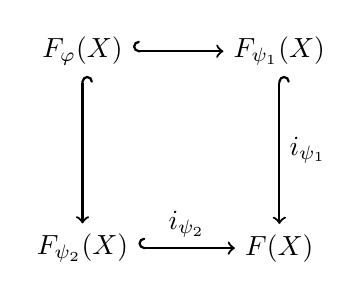
\begin{tikzpicture}[node distance=2.5cm, auto, thick]
            \node (A) {$F_\varphi(X)$};
            \node (B) [right of=A] {$F_{\psi_1}(X)$};
            \node (C) [below of=A] {$F_{\psi_2}(X)$};
            \node (D) [right of=C] {$F(X)$};
            \draw[right hook->] (A) to node {} (B);
            \draw[right hook->] (B) to node {$i_{\psi_1}$} (D);
            \draw[right hook->] (A) to node {} (C);
            \draw[right hook->] (C) to node {$i_{\psi_2}$} (D);
        \end{tikzpicture}
    };

    % Union
    \node[scale=2.3, opacity=0.3,color=white, yshift=-4.5cm, xshift=-2cm] at (current page.center) {%
        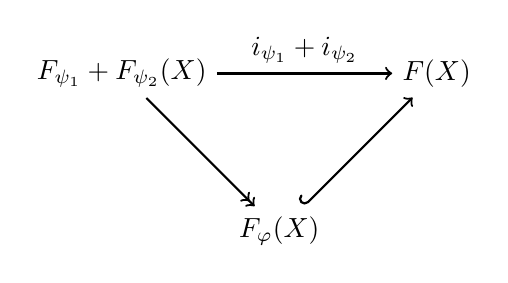
\begin{tikzpicture}[node distance=2cm, auto, thick]
            \node (A) {$F_{\psi_1} + F_{\psi_2}(X)$};
            \node (B) [right of=A] {};
            \node (C) [right of=B] {$F(X)$};
            \node (D) [below of=B] {$F_\varphi(X)$};
            \draw[->] (A) to node {$i_{\psi_1} + i_{\psi_2}$} (C);
            \draw[->>] (A) to node {} (D);
            \draw[right hook->] (D) to node {} (C);
        \end{tikzpicture}
    };


    %%%%%%%%%%%%%%%%%%%
    % Signature & Title
    %%%%%%%%%%%%%%%%%%%

    \node (jmeno) [anchor=north east, color=white, scale=2] at ($(current page.north east) - (1.2,0.5)$) {
        \begin{minipage}{1cm}
        \setlength{\parskip}{0.1cm}
        \hfill TOMÁŠ

        \hfill JAKL
        \end{minipage}
    };

    \draw[line width=1.5pt, color=white]
        ($(current page.north east) - (0.8,0.5)$) rectangle
        ($(current page.north east) - (3.8,3.3)$){};

    \node (cuni) [anchor=north east, color=white, scale=2.2] at ($(current page.north east) - (9.5,1)$) {
        \begin{minipage}{1cm}
        \librebaskerville
        CHARLES

        UNIVERSITY
        \end{minipage}
    };

    \draw[color=white,line width=2.5pt, -]
        ($(cuni.north west) - (0.45, 0)$) --
        ($(cuni.south west) - (0.45, 0)$);

    \node[anchor=north] (nadp) [yshift=-5.0cm, scale=4] at (current page.north) {%
        Coalgebras meet logic
    };

    \draw[decorate,decoration={brace,mirror,raise=6pt,amplitude=10pt}, thick]
        (nadp.north west)--(nadp.south west);
    \draw[decorate,decoration={brace,raise=6pt,amplitude=10pt}, thick]
        (nadp.north east)--(nadp.south east);

    \draw[decorate,decoration={brace,mirror,raise=6pt,amplitude=10pt}, thick]
        ($(nadp.north west)-(0.5,0)$)--($(nadp.south west)-(0.5,0)$);
    \draw[decorate,decoration={brace,raise=6pt,amplitude=10pt}, thick,xshift=1cm]
        ($(nadp.north east)+(0.5,0)$)--($(nadp.south east)+(0.5,0)$);


    %%%%%%%%%%%
    % Processes
    %%%%%%%%%%%

    \node (coalg1) at ($(nadp) + (-6,-5)$) {%
        \begin{minipage}{7cm}
        \setlength{\parskip}{0.5cm plus1mm minus3mm}
        \textbf{\Large Evolving systems:}

        \begin{itemize}
            \item Sequences of bits: 010110101110111101\dots
            \item (Nondeterministic) single-core computations.\newline
            \item Parallel/multiprocessor computations.
            \item Dynamical systems (the internet, financial systems, human thinking, \dots)
        \end{itemize}
        \end{minipage}
    };

    \node[opacity=0.8] (desc4) at ($(coalg1) + (2.5, -4.5)$) {
        \begin{minipage}{4cm}
        We still cannot satisfyingly reason about them. \footnotesize{(The hard part: sharing information, constant changes of the structure.)}
        \end{minipage}
    };


    \draw [very thick, rounded corners, draw=gray, dotted] ($(coalg1.north west)+(0.3,-3.7)$) rectangle ($(coalg1.south east)+(0.2,-0.2)$) {};

    \draw[decorate,decoration={brace,raise=10pt,amplitude=10pt}, very thick]
        (coalg1.north east)--(coalg1.south east);

    \draw[very thick, rounded corners, draw=gray, ->] (desc4.180) -| ($(coalg1.south west)+(1.0,-0.2)$);

    %%%%%%%%%%%%%%%%%%%%
    % Functor coalgebras
    %%%%%%%%%%%%%%%%%%%%

    \node [anchor=west] at ($(coalg1) + (10,2.3)$) {
        \begin{minipage}{4cm}
        \centering\textbf{\Large Coalgebras to\\
        rule them all:}
        \end{minipage}
    };

    \node (coalg2) [anchor=west] at ($(coalg1) + (10,0)$) {
        
\begin{tikzpicture}[remember picture, overlay, node distance=1.5cm]
        \node[scale=2] (funcA) {S};
        \node[scale=2] (funcB) [right of=funcA] {FS};
        \draw[->, very thick] (funcA) to node[above, scale=2] (f) {f} (funcB);
        \node (fBelow) [below of=f] {};

        \node[very thick, rounded corners, rectangle, draw=gray, dotted] [fit = (f) (fBelow) (funcA) (funcB)] {};
        \end{tikzpicture}
    };

    \node[anchor=west] (desc1) at ($(funcA) - (4.5,2.2)$) {
        \begin{minipage}{3cm}
            Possible states.
        \end{minipage}
    };

    \draw[->] (desc1) to node {} (funcA.220);


    \node[anchor=west] (desc2) at ($(funcA) - (2.5,3.5)$) {
        \begin{minipage}{3cm}
            A description of the process. % TODO
        \end{minipage}
    };

    \draw[->] (desc2) to node {} (f.220);

    \node[anchor=west] (desc3) at ($(funcB) - (1.5,3.0)$) {
        \begin{minipage}{3cm}
            A description of all accessible states.
            % TODO
        \end{minipage}
    };

    \draw[->] (desc3) to node {} (funcB.280);

    \draw[decorate,decoration={brace,mirror,raise=6pt,amplitude=10pt}, very thick]
        ($(f.south west) - (4,4.5)$)--($(f.south east)+(3,-4.5)$);

    %%%%%%%%%%%%%
    % Modal logic
    %%%%%%%%%%%%%

    \node (modal) [anchor=north] at ($(coalg1.south) - (0,4.5)$) {
        \begin{minipage}{6cm}
        \setlength{\parskip}{0.5cm plus1mm minus3mm}
        \textbf{\Large Modal logic}

        Is a formal language suitable for reasoning about dynamical (computer) systems.

        Modal logic allow us to talk about future states of systems by adding two new
        language constructs:
        \vspace{-0.5em}
        \begin{itemize}
        \item \textbf{\large Possibility -- $\Box P$: } Property $P$ holds in all future states.
        \item \textbf{\large Certainty -- $\Diamond P$: } There is a future state where the property $P$ holds.
        \end{itemize}
        \end{minipage}
    };

    \draw[decorate,decoration={brace,mirror,raise=6pt,amplitude=10pt}, thick]
        (modal.south west)--(modal.south east);


    %%%%%%%%%%%%%%%%%%%%
    % Translation schema
    %%%%%%%%%%%%%%%%%%%%

    \node (robot1) [scale=1.2] at ($(coalg2) - (-0.0,8.5)$) {
        Procedure \textbf{IS} in a deadlock \textbf{OR} will be in the next step.
        % TODO
    };

    \node (robot2) [scale=2] at ($(robot1) - (0,3.0)$) {
        $S\overset{f}{\longrightarrow} FS \models~ \bot\,\text{ OR }\, \Box \bot$
    };

    \draw[->] ($(robot1) - (4,0.5)$) to node {} ($(robot2) - (3.0,-0.6)$);
    \draw[->] ($(robot1) - (2.4,0.5)$) to node {} ($(robot2) - (0.8,-0.6)$);
    \draw[->] ($(robot1) - (1,0.5)$) to node {} ($(robot2) - (-0.5,-0.6)$);
    \draw[->] ($(robot1) - (-3.5,0.5)$) to node {} ($(robot2) - (-3.0,-0.6)$);

    \draw[thick, draw=gray, snake=zigzag]
        ($(robot1.north west) + (-0.25, +0.5)$) --
        ($(robot1.north east) + ( 0.25, +0.5)$) --
        ($(robot1.south east) + ( 0.25, -0.5) - (0, 3.0)$) --
        ($(robot1.south west) + (-0.25, -0.5) - (0, 3.0)$) --
        ($(robot1.north west) + (-0.25, +0.5)$);

    \node[anchor=south east,scale=1.5] at ($(current page.south east) - (1.5,-2.2)$) {
        \begin{minipage}{5cm}
        \centering
        \bf
        A discovery of the right combination of a language and structures can completely change the way we think about software!
        \end{minipage}
    };


    %%%%%%%%
    % Arrows
    %%%%%%%%

    \draw[->, shorten >=1cm, shorten <=1cm, line width=1.8pt] (coalg1.0) to node[above] {%
        \begin{minipage}{4cm}
        \centering They share the same\\ structure!\vspace{1em}
        \end{minipage}%
    } (coalg2.180);

    \draw[->, shorten >=0.5cm, shorten <=1cm, line width=1.0pt]
        (modal.270) --
        ($(modal.270) - (0,2)$) -|
        ($(robot2.270) - (4.5,0)$);

    \node at ($(modal.270) - (-2.8,2.5)$) {
        Gives an appropriate language!
    };

    \draw[->, line width=1.0pt]
        ($(f.270) - (0.5,5.5)$) --
        ($(f.270) - (0.5,7.0)$);
\end{tikzpicture}
\end{document}

